\documentclass[sn-nature]{sn-jnl}

\usepackage{graphicx}
\usepackage{amsmath}
\usepackage{float}

\unnumbered% unnumbered section heads (Nature-style)

\begin{document}
\title[Low-carbon lifestyles and broad emission reductions]{Low-carbon lifestyles show broadly lower emissions without automatic rebound}

\author*[1]{\fnm{David} \sur{Andersson}}\email{david.andersson@chalmers.se}

\author[2,3]{\fnm{Jakob} \sur{Enlund}}\email{jakob.enlund@lnu.se}

\author[4]{\fnm{Jonas} \sur{Nässén}}\email{jonas.nassen@chalmers.se}

\affil*[1]{\orgdiv{Chalmers Next Labs}, \orgname{Chalmers University of Technology}, \orgaddress{\city{Gothenburg}, \country{Sweden}}}

\affil[2]{\orgdiv{Department of Economics and Statistics}, \orgname{Linnaeus University}, \orgaddress{\city{Växjö}, \country{Sweden}}}

\affil[3]{\orgdiv{Department of Economics and Statistics}, \orgname{University of Gothenburg}, \orgaddress{\city{Gothenburg}, \country{Sweden}}}

\affil[4]{\orgdiv{Department of Environmental and Energy Sciences}, \orgname{Chalmers University of Technology}, \orgaddress{\city{Gothenburg}, \country{Sweden}}}

\abstract{Low-carbon lifestyles are a central demand-side option for climate mitigation, but the money they free up is widely assumed to be re-spent on other emission-intensive consumption, eroding around half of their estimated potential---an assumption scarcely tested empirically. We link bank-transaction, registry, and survey data for 1,296 Swedish single-adult households and estimate emission differences associated with car-free, flight-free, and meat-free living, decomposed into direct (within-domain) and indirect (all other consumption) components. Car-free and flight-free households show direct savings of $-$1.26 and $-$1.84 tCO$_2$e per person-year and total differences of $-$1.51 and $-$2.06 tCO$_2$e (both {\mathversion{normal}$p < 0.001$}); meat-free diets $-$0.47 tCO$_2$e ({\mathversion{normal}$p = 0.084$}). Despite large financial savings, no lifestyle group shows higher indirect emissions, and for both mobility lifestyles observed indirect emissions fall significantly below proportional re-spending benchmarks. Stronger environmental self-identity predicts lower emissions across the rest of the budget: environmentally motivated adopters achieve the broadest reductions. These results challenge automatic rebound assumptions and suggest that motivation shapes spending patterns.}

\keywords{rebound effect, carbon footprint, environmental self-identity, demand-side mitigation, household consumption}

\maketitle
Reducing car dependence, flying less, and eating plant-based rank among the highest-impact climate actions available to households in high-income countries \citep{IPCC_AR6_WG3_2022,Creutzig2022,Wynes2017}. Yet a person who gives up their car is often told that the effort is partly self-defeating: the money no longer spent on the car will be spent on something else, and the emissions embodied in that new spending will offset the original saving \citep{hubacek2011net,Berkhout2000,SorrellDimitropoulos2008,Hertwich2005,sorrell2020,Reimers2022}. The reasoning descends from supply-side efficiency analysis where cheaper energy services raise demand \citep{SorrellDimitropoulos2008}, and is now standard in household-footprint and scenario studies \citep{Chitnis2013,Bjelle2018,Niamir2020}. How much of the emission saving survives depends largely on the assumed re-spending pattern: in a recent global assessment, re-spending at prevailing consumption patterns offsets 46\% of the savings from combined lifestyle changes, and only a best case in which all savings flow to the least carbon-intensive services limits the loss to 7\% \citep{guan2025unlocking}. National studies report offsets of roughly 40--60\% under average re-spending \citep{ChitnisSorrell2015,Bjelle2018}, and up to or above 100\% for some food-related measures \citep{Chitnis2014}. 

But living without a car, rather than owning a more fuel-efficient one, is not a marginal adjustment: it comes with different practices---where one lives, shops, and spends weekends. Furthermore, people live without cars, flights, and meat for many reasons---prices, access to substitutes, urban living, fear of flying, health, animal welfare. In cases where the low-carbon lifestyle is primarily motivated by environmental concern, re-spending the savings on something equally polluting seems counterintuitive. Environmental self-identity (ESI)---the extent to which people see environmentally friendly behaviour as part of who they are---predicts instead a positive spillover from pro-environmental behaviour in one domain to another \citep{VanDerWerff2013,WhitmarshONeill2010,udall2021}, though experiments and surveys find both consistency and its opposite, moral licensing \citep{Truelove2014,thogersen1999spillover,Merritt2010,Blanken2015,Nilsson2017}. What adopters actually do with the money has not been directly observed: existing rebound estimates are simulated or rely on self-reported spending \citep{ottelin2024rebound}.

We provide, to our knowledge, the first individual-level test of the re-spending assumption based on observed rather than simulated or self-reported consumption. We link bank-transaction records covering close to the full consumption budget \citep{AnderssonNassen2023,trendl2023} with registry data and survey responses for 1{,}296 participants recruited through a register-based random-invitation frame of Swedish single-adult households. This also represents the population-level data that indirect-effect tests have lacked \citep{exadaktylos2021energy}. We compare households established in a lifestyle---living without a car, avoiding air travel, or following a meat-free diet---with demographically similar households that are not: if adopters re-spend the money their lifestyle frees up, the resulting consumption should be recorded as higher spending and emissions outside the focal domain. For each contrast, we estimate adjusted annual emission differences, separate focal-domain emissions from emissions in all other consumption, benchmark the latter against full proportional re-spending, and test whether the pattern varies with ESI.

Car-free and flight-free households have substantially lower total emissions than their comparison groups; the meat-free estimate is smaller and less precise. None of the three groups has higher estimated emissions outside its focal domain, and for the two mobility contrasts the observed estimates fall below the proportional re-spending benchmarks. Stronger ESI is associated with lower non-focal emissions overall, but the adopter--non-adopter gap does not widen with ESI---the stricter test, since high-ESI households may simply emit less regardless of lifestyle.

\begin{figure}[htbp]
\centering
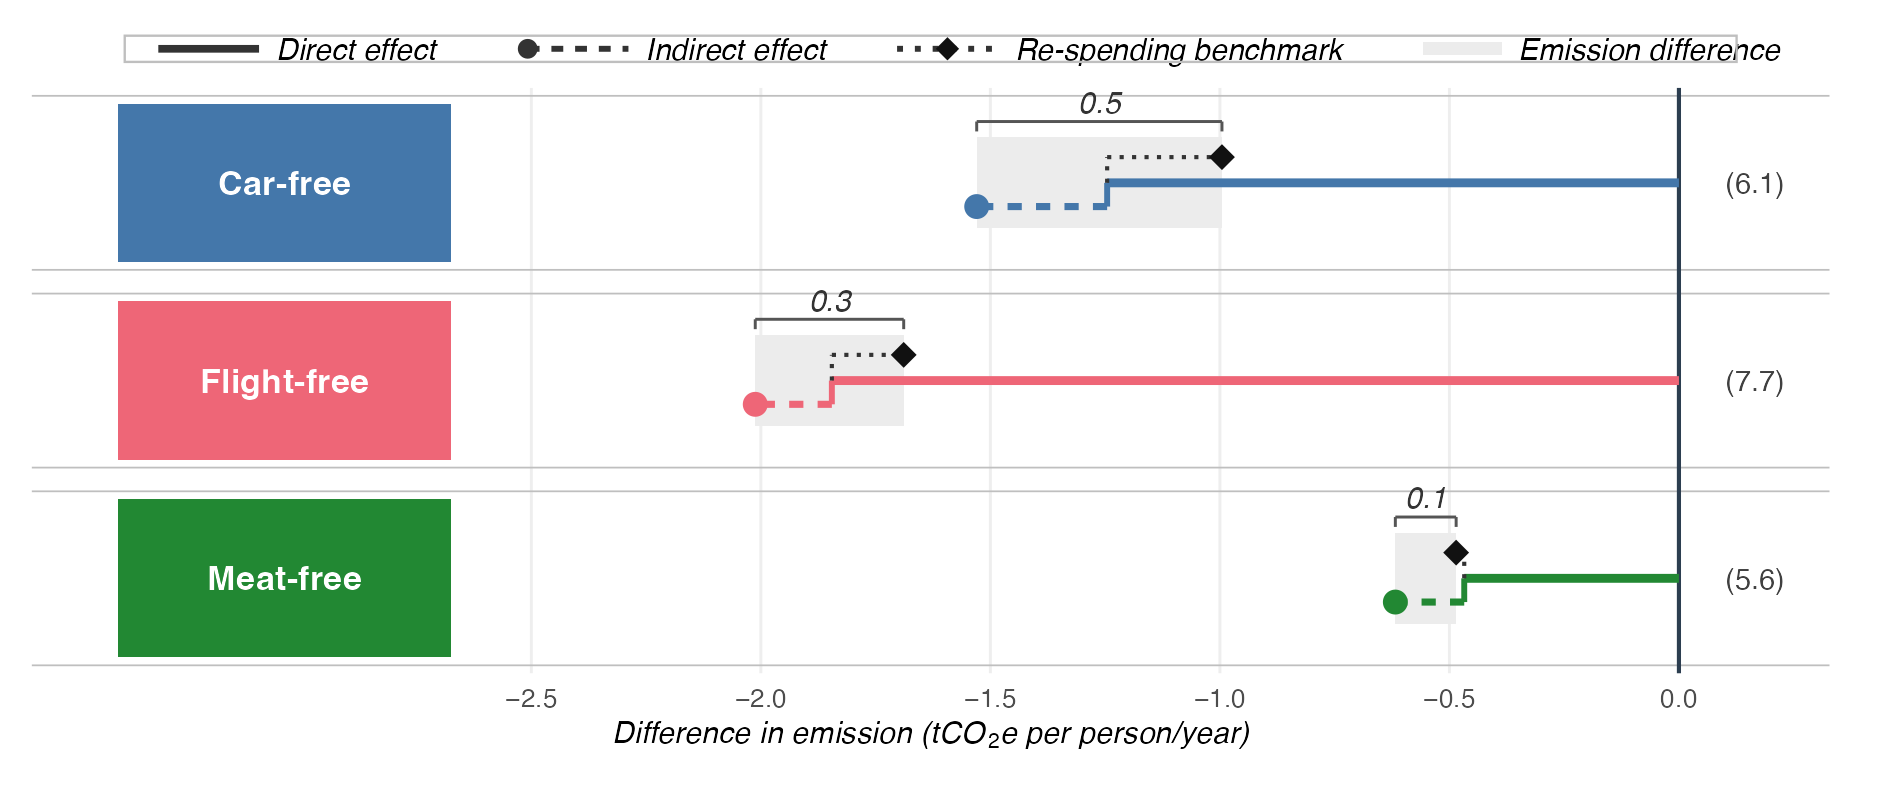
\includegraphics[width=0.95\textwidth]{../results/Waterfall_pres_main.png}
\caption{\textbf{Large direct emission reductions; indirect emissions fall below the re-spending benchmark.} Regression-adjusted emission differences between lifestyle adopters and demographically similar non-adopters (tCO$_2$e per person-year). Solid segments show direct (focal-domain) savings, dotted segments show indirect (all other domains) effects. The marker indicates the re-spending benchmark: the expected indirect level if adopters proportionally reallocate freed focal-domain spending to non-adopters' non-focal consumption. For car-free and flight-free households, indirect emissions fall left of the benchmark, below what proportional re-spending would predict; for meat-free households, the observed and benchmark values are both close to zero. Numbers in parentheses show corresponding non-adopter group mean footprints. Models control for income, sex, age group, education, children, housing type, major city indicator, and log population density.}
\label{fig_main}
\end{figure}

\begin{figure}[htbp]
\centering
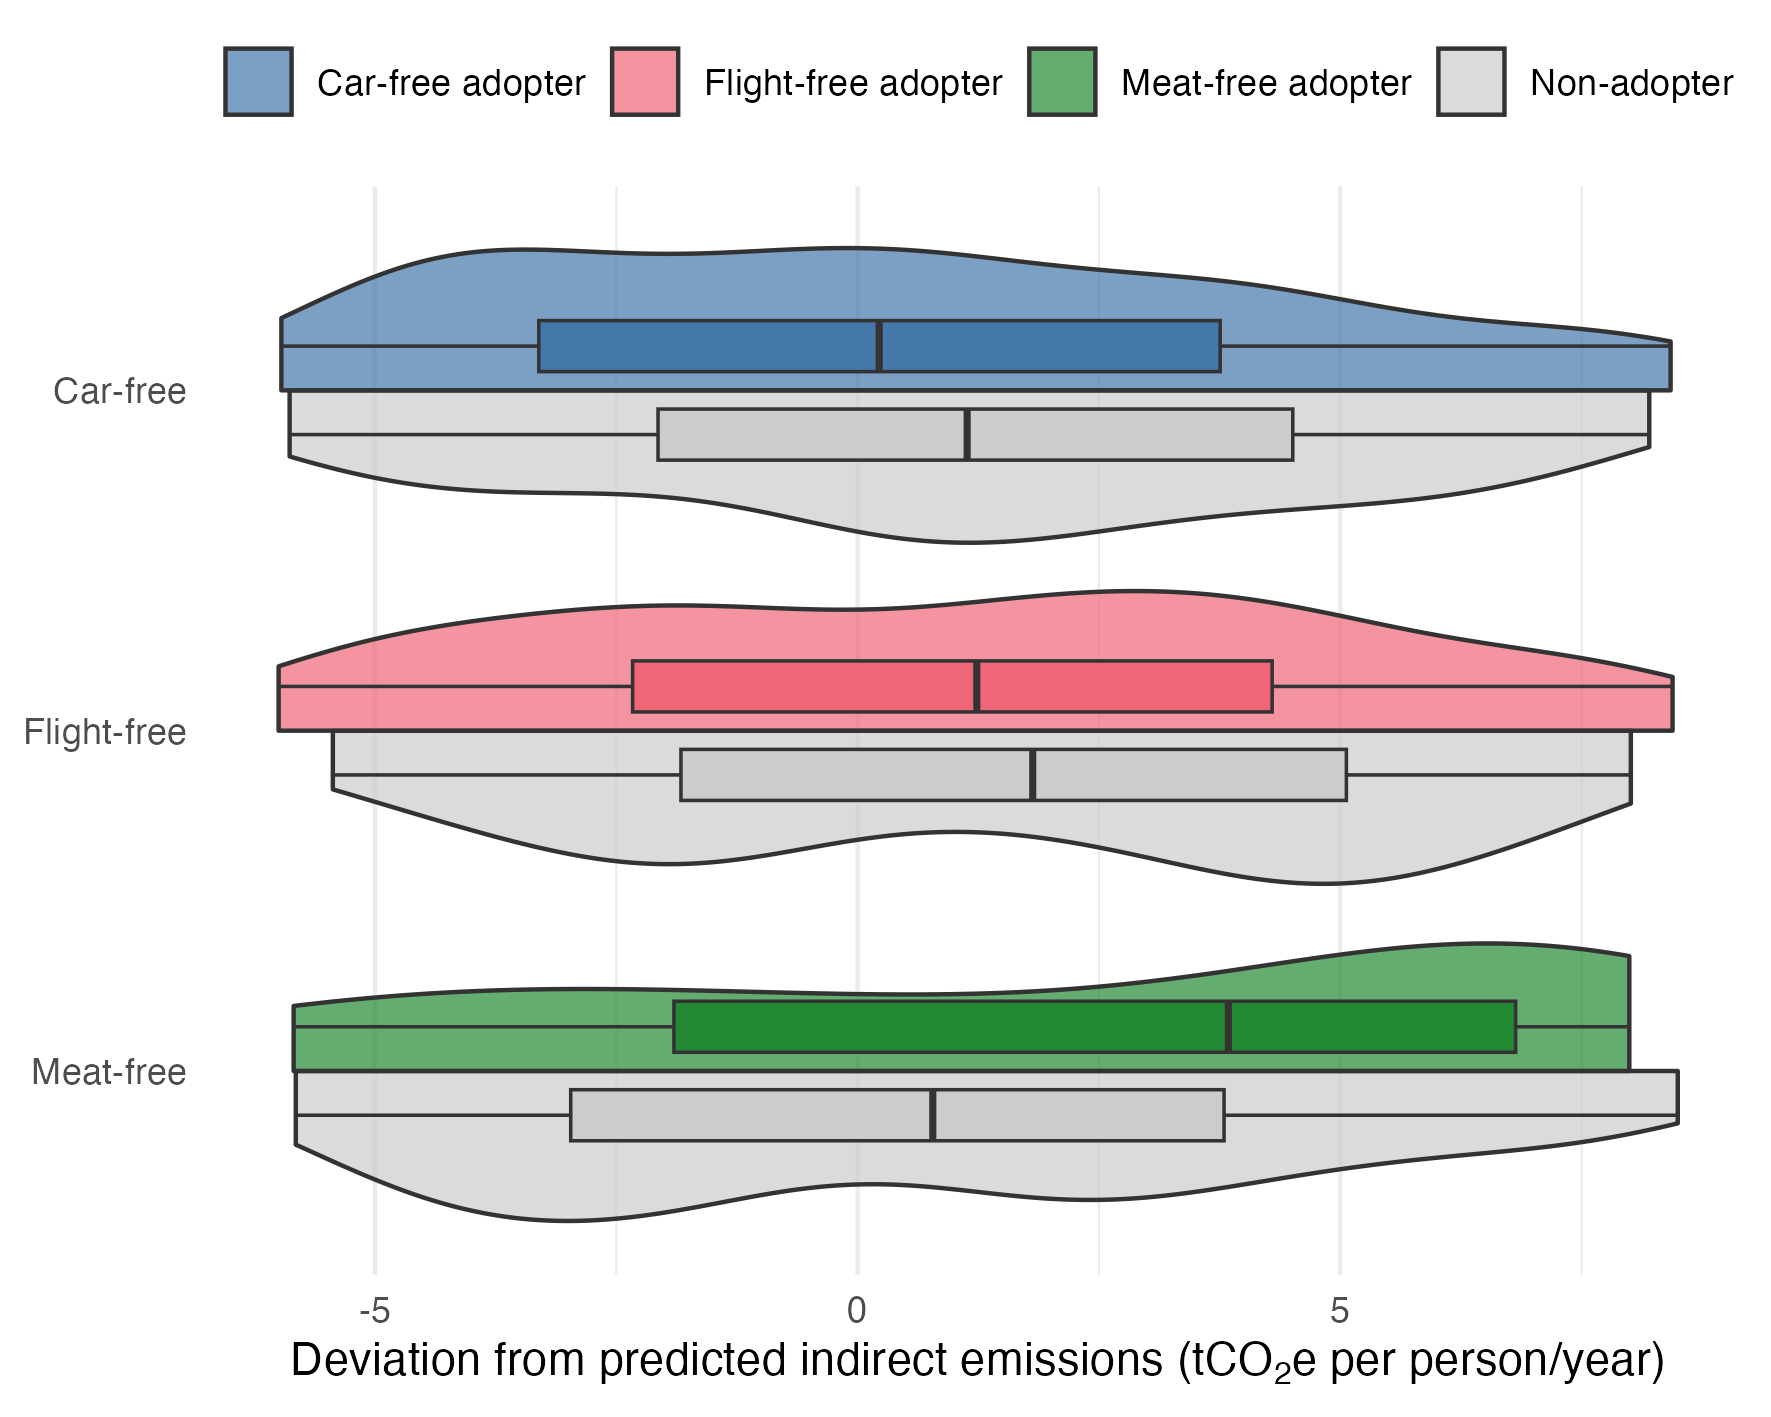
\includegraphics[width=0.95\textwidth]{../results/Residuals distribution.png}
\caption{\textbf{Car-free and flight-free adopters show a systematic left-shift in indirect emissions.}
Each panel shows a split violin comparing the distribution of residualised indirect (non-focal) CO$_2$e emissions (tCO$_2$e per person-year) for lifestyle adopters (lifestyle colour) and non-adopters (grey). Residuals are the difference between a household's measured indirect emissions and the level predicted by its demographic profile (income, sex, age group, education, children, housing type, major city indicator, and population density); zero means measured emissions equal the model prediction, and negative values mean a household emits less than its profile predicts. Wider sections of each violin indicate more households at that emission level; embedded box plots show median and interquartile range. A leftward shift indicates systematically lower indirect emissions than demographically similar non-adopters. Kolmogorov–Smirnov tests confirm a significant left-shift for car-free (\textit{p} = 0.027) and flight-free households (\textit{p} = 0.007), but no significant shift for meat-free households (\textit{p} = 0.060), indicating that the indirect pattern reflects a broad-based difference in non-focal consumption rather than the influence of outliers.}
\label{fig_violin}
\end{figure}

\begin{figure}[htbp]
\centering
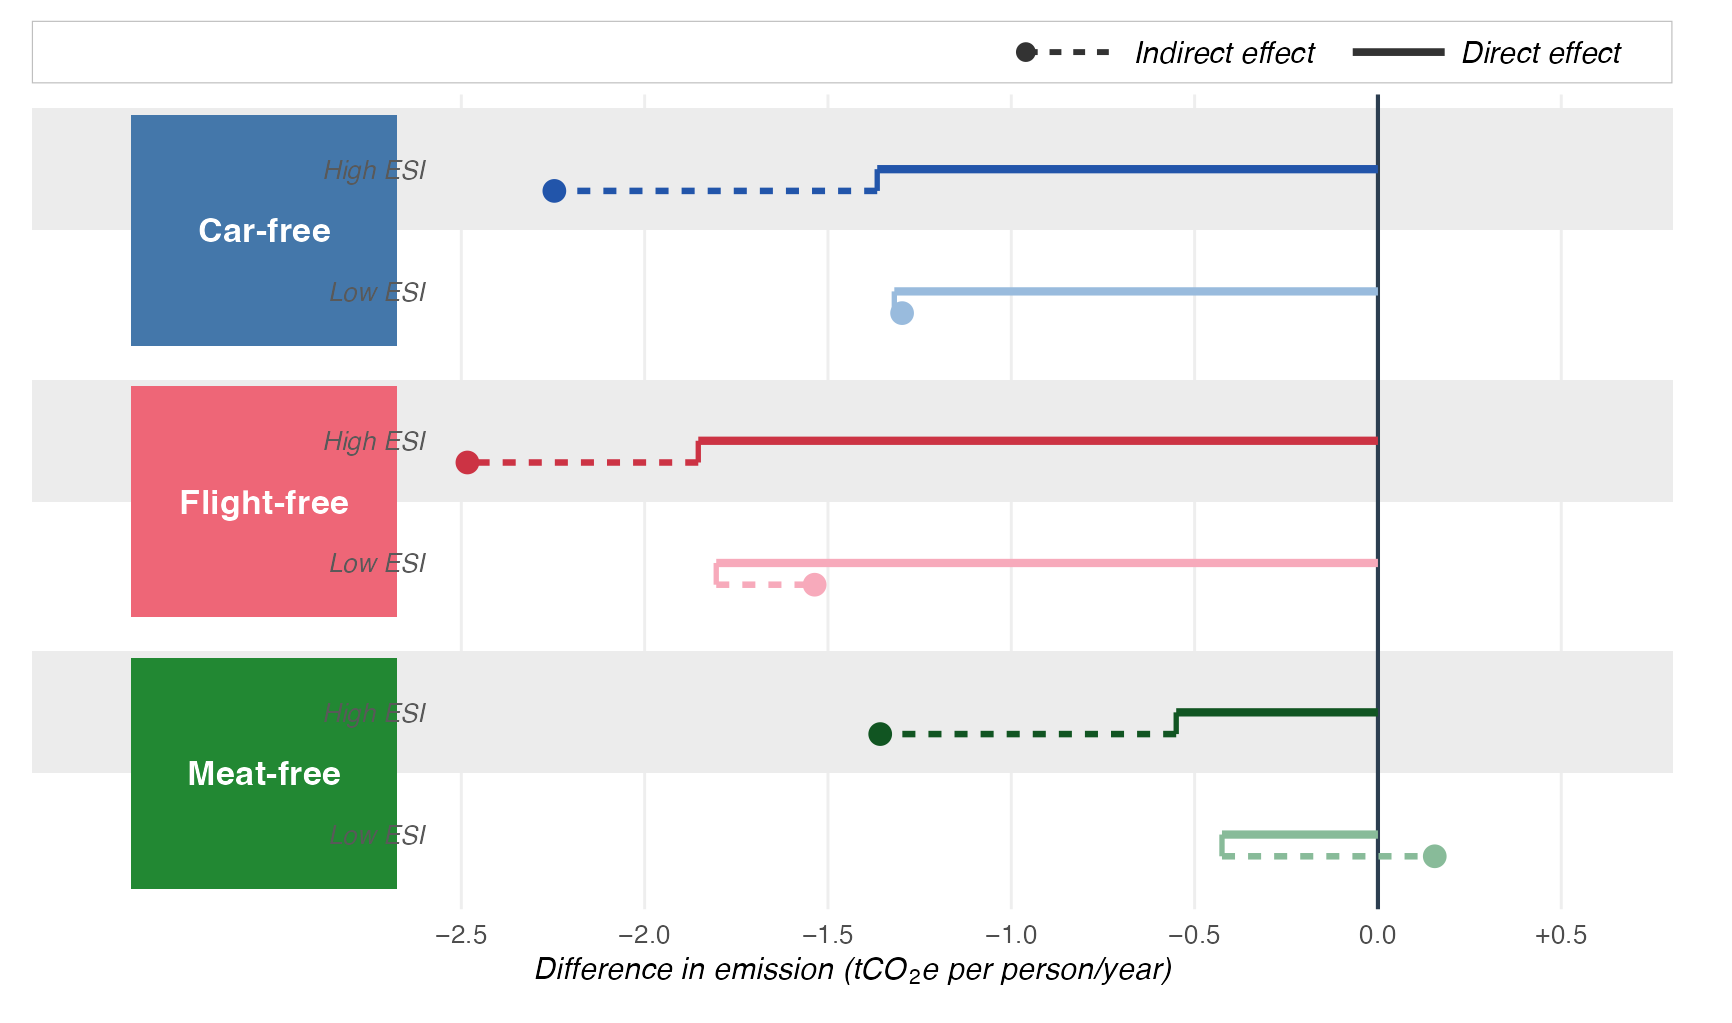
\includegraphics[width=0.95\textwidth]{../results/Waterfall_pres_esi.png}
\caption{\textbf{Environmental self-identity stratifies the indirect emission pattern.}
Regression-adjusted emission differences at high ESI ($+1$~SD; dark shade) and low ESI ($-1$~SD; light shade) relative to an ESI~$= 0$ non-adopter reference (zero at right); segments extending left denote lower emissions than non-adopters. For each contrast, the solid segment shows the direct saving and the dotted segment extends from the direct endpoint to the indirect endpoint, with a marker indicating the total (direct plus indirect) effect. At high ESI (dark shades), the total-effect markers consistently fall further left than the direct endpoint, indicating that environmentally motivated adopters achieve broad-based additional reductions beyond the focal domain; at low ESI (light shades), markers fall near or to the right of the direct endpoint, consistent with slightly offsetting indirect effects. Direct and indirect effects are derived from multivariate regressions adjusting for income, sex, age group, education, children, housing type, major city indicator, and population density. 95\% confidence intervals are omitted for clarity (Supplementary Information, Section~S7). Models as in Fig.~\ref{fig_main}.}
\label{fig_esi}
\end{figure}

\section{Results}
\subsection{Sample characteristics}
The analytical sample comprised 1{,}296 single-adult households meeting data quality criteria (Methods). The descriptive summaries of the registry and the survey data are reported in Supplementary Information, Section~S2. The mean annual footprint was approximately 5.37~tCO$_2$e per person. For context, official consumption-based statistics attribute close to 5~tCO$_2$e per person-year to Swedish household consumption excluding emissions related to government spending \citep{naturvardsverket_konsumtion_2025}. The two numbers are not directly comparable: our sample consists of single-adult households, which lack the household economies of scale that lower per-capita footprints in the general population, and our aviation intensity incorporates non-CO$_2$ high-altitude effects that the national model omits (Supplementary Information, Section~S3). Both differences are expected to place our estimate somewhat above the population-wide household average, consistent with what we observe.

\subsection{Average direct and indirect differences}
As illustrated in Fig.~\ref{fig_main}, living car-free and avoiding air travel are associated with regression-adjusted total emission differences of $-$1.51 and $-$2.06~tCO$_2$e per person-year, respectively (both $p < 0.001$). Following a meat-free diet is also associated with lower emissions than in similar households---a total difference of $-$0.47~tCO$_2$e---but does not reach significance in this sample ($p = 0.084$).

For car-free households, the direct component is $-$1.26~tCO$_2$e and the indirect component is $-$0.25~tCO$_2$e ($p = 0.39$). For flight-free households, the direct component is $-$1.84~tCO$_2$e and the indirect component is $-$0.21~tCO$_2$e ($p = 0.32$). For meat-free households, the direct component is $-$0.47~tCO$_2$e ($p < 0.001$), while the indirect component is small and non-significant ($-$0.01~tCO$_2$e, $p = 0.98$). Hence, across the two mobility-related lifestyles, indirect effects are negative (in the spillover direction). The indirect point estimates are individually imprecise, but they are not incidental quantities: by construction they capture the entire difference between the total and direct effects, and two complementary tests---the distributional comparison below and the re-spending benchmark in the next section---both indicate that the absence of offsetting is systematic rather than noise. Kolmogorov--Smirnov tests confirm that the indirect pattern reflects a broad-based difference in non-focal consumption rather than the influence of outliers: the full distribution of indirect emissions is shifted toward lower values for car-free ($p = 0.027$) and flight-free households ($p = 0.007$), while the shift for meat-free households falls just short of conventional significance ($p = 0.060$; Fig.~\ref{fig_violin}). 

\subsection{Proportional re-spending benchmark}
As a stylized benchmark, we approximate indirect emissions under proportional re-spending: we first estimate the regression-adjusted financial saving in the focal domain, and then multiply this saving by the comparison group's mean emission intensity (kg~CO$_2$e per SEK) of the non-focal consumption bundle (Methods). 

For car-free households, the benchmark predicts an indirect increase of $+$0.256~tCO$_2$e from proportional re-spending of freed resources, whereas the observed indirect estimate is $-$0.255~tCO$_2$e, a gap of $-$0.511~tCO$_2$e. For flight-free households, the benchmark predicts $+$0.151~tCO$_2$e, against an observed $-$0.212~tCO$_2$e, a gap of $-$0.363~tCO$_2$e. For meat-free households, the benchmark predicts $-$0.008~tCO$_2$e (because regression-adjusted focal-domain spending is higher rather than lower for non-meat households), while the observed indirect effect is $-$0.005~tCO$_2$e. For car-free and flight-free households, one-sided tests reject a rebound as large as the proportional re-spending benchmark ($p = 0.041$ and $p = 0.045$; Supplementary Information, Section~S9.1), so the observed shortfall relative to the benchmark is statistically robust rather than merely descriptive.

\subsection{The role of environmental motivation in indirect emission patterns}
As noted earlier, the average indirect differences described above pool households with different environmental motivation. Motivation could shape the indirect pattern through two distinct channels, and we test each. First, environmental identity may predict less carbon-intensive spending across the whole budget, for adopters and non-adopters alike---a main effect of ESI. Second, adoption itself may catalyse or strengthen behaviour, which would correspond to the indirect-emission gap between adopters and non-adopters widening with higher ESI---what we term principled spillover \citep{VanDerWerff2013,Truelove2014}. Statistically, the first channel is the ESI main effect and the second is the ESI~$\times$~lifestyle interaction: under purely mechanical rebound the interaction should be zero; under principled spillover it should be negative, with adopters having even lower emissions at higher ESI.

The first analysis predicts adopters' indirect emissions at low ($-$1~SD), mean, and high ($+$1~SD) ESI, and compares each with a non-adopter at average ESI (Fig.~\ref{fig_esi}). This gradient tracks environmental identity itself. Each standard-deviation increase in ESI is associated with lower indirect emissions in all three models ($p = 0.061$, $0.035$, and $0.003$ for the car, flight, and diet models, respectively). As a result, car-free and flight-free adopters with strong environmental identity emit 0.64 and 0.65~tCO$_2$e less across the rest of their budget than the ESI-neutral reference, whereas adopters with weak identity sit near or slightly above it ($+$0.12 and $+$0.21~tCO$_2$e, respectively).

Category-level results tell the same story. Relative to the same ESI-neutral reference, adopters with strong environmental identity show reductions spread broadly across most non-focal categories. Adopters with weak identity show a more mixed pattern. Where their emissions run higher, they concentrate in the other high-carbon domains: low-ESI car-free households show elevated aviation emissions, and low-ESI flight-free households show elevated car and public transport emissions (Fig.~\ref{fig_category}; Supplementary Information, Section~S12). Supplementary Information, Section~S7 shows these patterns as continuous predicted emission levels across the full ESI range.

\begin{figure}[htbp]
\centering
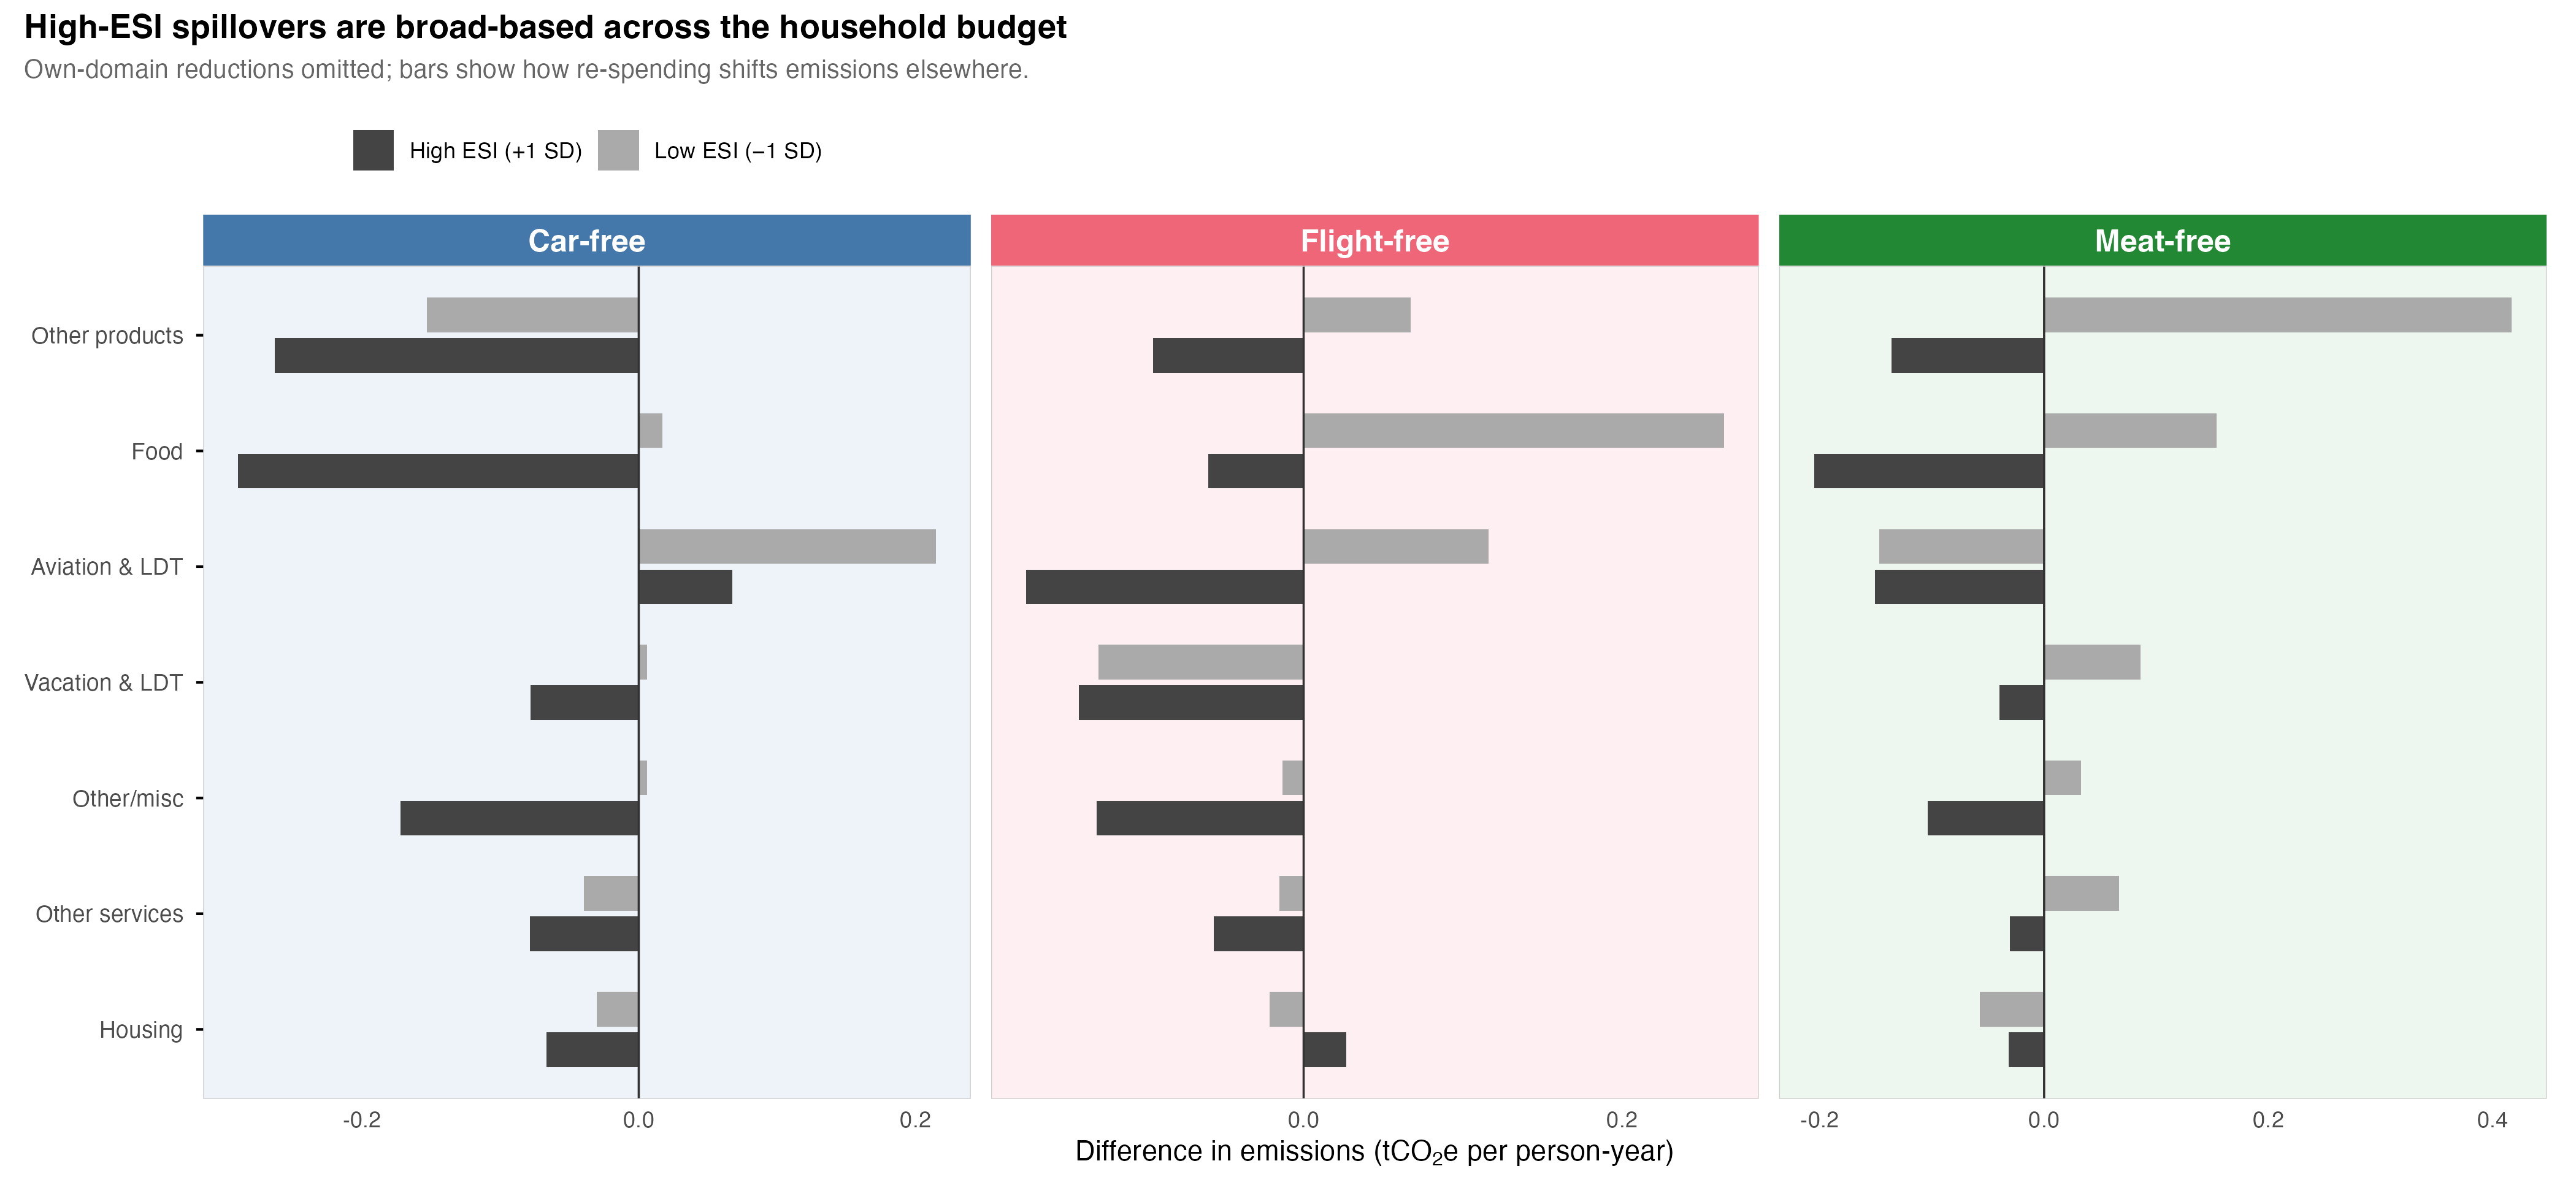
\includegraphics[width=\textwidth]{../results/category_decomposition_esi.png}
\caption{\textbf{High-ESI adopters occupy broad-based lower-emission positions; low-ESI adopters' positions concentrate in substitution channels.}
Regression-adjusted emission differences at high ESI ($+1$~SD; dark bars) and low ESI ($-1$~SD; light bars) for each broad consumption category, relative to an ESI~$= 0$ non-adopter reference; all panels share the same x-axis scale. Bars extending left of zero indicate an emission reduction in that category; bars extending right indicate an increase. Own-domain categories (car and public transport for car-free, aviation for flight-free, food for meat-free) are omitted from this panel for visual clarity and are shown in full in Fig.~\ref{fig_main}. For high-ESI adopters (dark bars), reductions are distributed broadly and coherently across most categories. For low-ESI adopters (light bars), patterns are more mixed and notably include positive bars in other focal domains: car-free low-ESI households show elevated aviation emissions, and flight-free low-ESI households show elevated car and public transport emissions—consistent with substitution toward the other high-carbon domains that high-ESI adopters appear to restrain. Panels correspond to Car-free (blue), Flight-free (coral), and Meat-free (green) lifestyle contrasts. Models as in Fig.~\ref{fig_main}.}
\label{fig_category}
\end{figure}

The second, stricter test does not support principled spillover. The interaction terms are not significant for any lifestyle, on either indirect CO$_2$e ($p = 0.60$, $0.42$, and $0.97$ for the car, flight, and diet models) or indirect spending (Supplementary Information, Section~S7). The ESI gradient described above therefore comes from identity itself, not from identity amplifying the effect of adoption.

The interaction estimates are nonetheless directionally suggestive for the two mobility lifestyles: the adopter slope against ESI is slightly steeper than the non-adopter slope (interaction coefficients $-$99 and $-$129~kg\,CO$_2$e per SD), the pattern principled spillover would predict. The effect is, however, small and statistically indistinguishable from zero. This is expected even if the mechanism is real: interactions are second-order effects, and detecting them reliably requires several times the sample needed for a main effect. Establishing principled spillover would require clear, robust negative ESI~$\times$~lifestyle interactions. That criterion is not met here, so we rest our ESI claims on the precisely estimated main effect rather than on moderation.

\section{Discussion}
Rebound theory postulates that money saved in one domain is mechanically re-spent across the rest \citep{Berkhout2000,sorrell2020}. Our findings say otherwise. Car-free and flight-free households free up more money than their comparison groups, yet emit less across the rest of their budget, and their observed indirect emissions fall well short of proportional re-spending benchmarks. Nor does the freed money surface elsewhere in consumption: adopters' non-focal spending is, if anything, lower as well (Supplementary Information, Section~S7). These spending estimates are imprecise, but they point toward saving rather than re-spending---the margin that budget-closure models hold fixed. Saved money may of course be consumption merely postponed, which our observation window cannot fully rule out, although the extended-window analysis finds persistent restraint rather than deferral (Supplementary Information, Section~S6.4). Environmental self-identity offers one explanation: households with stronger ESI spend their budget on less carbon-intensive goods, regardless of lifestyle. Even adopters with weak identity show no broad rebound, but their higher spending tends to surface in more climate-intensive substitution channels (Fig.~\ref{fig_category}). Adopting a low-carbon lifestyle appears to reshape surrounding practices and consumption patterns.

Stronger identity is associated with lower indirect emissions across the board, but we find no sign that adoption carries extra weight at high ESI: the adopter--non-adopter gap does not widen with identity, possibly for lack of statistical power. What is robust is the main association---environmentally identified households show lower non-focal emissions in general---and that alone matters for how aggregate re-spending is represented.

More broadly, our results are consistent with and strengthen our previous findings: no rebound in a self-selected, environmentally motivated sample \citep{AnderssonNassen2023}, and zero direct rebound among car buyers changing to ``green''-labelled cars, whereas buyers who improved their fuel efficiency by a similar margin, but without the ``green'' label, rebounded by roughly 30\% \citep{andersson2019estimating}. Both studies hinted at motivation but could not isolate it. Our results contrast with recent survey-based evidence that rebound flattens footprint differences between car-free households and car owners \citep{ottelin2024rebound}; a plausible source of the divergence is measurement, since self-reported expenditure is subject to recall and social-desirability error that transaction records avoid.

These findings speak directly to how demand-side mitigation is quantified. Observed indirect emissions fall substantially below proportional re-spending benchmarks for car-free and flight-free households, with distributional tests confirming the pattern (Supplementary Information, Section~S8); for meat-free households, benchmark and observed values are both close to zero, consistent with the smaller financial savings involved. Prospective input--output and integrated assessment studies estimate the mitigation potential of lifestyle changes while either imposing proportional re-spending through budget closure with representative-agent demand systems \citep{Chitnis2013,Deaton1980,Gillingham2016,Niamir2020,Bjelle2018,grabs2015rebound}, or leaving rebound unquantified as an acknowledged limitation \citep{cap2025reduction}. In such closures, rebound is automatic---it follows from the model's construction rather than from evidence: money not spent in one domain has nowhere to go but other consumption, since saving is typically held fixed, and it is reallocated according to the average household's spending pattern. Our results offer empirical guidance for both choices: for mobility-related lifestyle changes, undiscounted mitigation potentials appear closer to observed behaviour than estimates corrected by proportional rebound. The results also address the recognised gap that models represent \emph{what} changes but not \emph{who} changes or why \citep{scherer2025lifestyle,vandenberg2019improved}: environmental self-identity is a measurable trait that predicts non-focal emission intensity, making motivational composition a tractable dimension for the consumer heterogeneity these frameworks increasingly seek to represent---and suggesting that expenditure elasticities estimated on representative households mask motivation-correlated heterogeneity in how freed budget is re-spent. To the extent that our findings hold beyond voluntary adopters, the stakes are substantial: in the global assessment above, assumed re-spending alone erases 4.8~GtCO$_2$e or nearly half of the estimated potential of lifestyle changes among high-consuming households \citep{guan2025unlocking}.

Several limitations should be noted. Because the analysis is observational and cross-sectional, all estimates reflect population-based associations and should not be interpreted as causal effects of adopting a behaviour. Individuals who live without a car, avoid air travel, or follow meat-free diets likely differ from their comparison groups on dimensions not fully captured by observed controls, including preferences and built-environment access beyond population density and urbanity. Similarly, environmental self-identity is self-reported, and identity and behaviour plausibly reinforce one another over time, so the ESI gradients should be read as associations rather than one-directional influences. The restriction to single-adult households simplifies the attribution of spending to a single household budget, but limits generalizability.

At the same time, the cross-sectional design has a compensating strength for the spillover question. Negative spillover and moral licensing are documented largely in experimental and short-run settings where a recently adopted behaviour is salient \citep{Merritt2010,Blanken2015}; if compensatory responses are most pronounced during behavioural transitions, our design---observing established rather than newly induced behaviours---would better capture the settled phase most relevant for long-run mitigation.

The Swedish cultural context deserves particular attention. Sweden combines comparatively high environmental concern and carbon literacy with a long-standing public discourse emphasising individual responsibility for one's carbon footprint \citep{eib_climate_2021,naturvardsverket_2023,oecd_sweden_2025}---reflected in the emergence of \textit{flygskam} (``flight shame''), which originated in Sweden in 2018 \citep{wolrath2019grounded}. These norms may reinforce the behavioural consistency associated with environmental self-identity, making the ESI gradient observed here partly context-dependent. To the extent that environmental self-identity is shaped by social discourse and norm formation rather than fixed individual disposition \citep{vanderwerff2014past,nyborg2016social}, the motivational composition of a population is itself a potential object of policy. Our cross-sectional design cannot test this dynamic, but it implies that the aggregate indirect emissions accompanying lifestyle change may depend on the normative context in which adoption occurs.

Measurement limitations of expenditure-based footprinting---imperfect transaction categorisation and the inability to distinguish within-category intensity variation---are detailed in Methods; both work against detecting the indirect reductions we report, making our estimates conservative. The meat-free contrast additionally rests on self-reported diet for both group definition and food-intensity calibration; its direct estimate is therefore measured with more error than the mobility contrasts---whose focal quantities are observed in transaction and registry data---and is plausibly attenuated as a result. Likewise, a single 12-month window pools incidental with committed non-flyers, biasing the flight-free estimate toward zero. Under a longer confirmatory window requiring zero air travel throughout, the flight-free indirect reduction strengthens to $-$0.46~tCO$_2$e ($p = 0.027$), supporting genuine restraint over deferred consumption; car-free and meat-free results are stable (Methods; Supplementary Information, Section~S6.4).

Despite these limitations, the results provide rare empirical evidence that low-carbon lifestyles are not systematically offset by higher emissions elsewhere in a population-based sample. If lifestyle transitions occur at scale, the net climate benefit may depend not only on the direct emissions avoided but also on whether adoption is driven by environmental concern or policy alone. Future research should examine whether similar no-rebound patterns hold in multi-person households, and whether cross-national comparisons across contexts with different environmental norms can identify how cultural and social context shapes net effects in different groups. A complementary question is whether re-directed spending re-emerges when cost savings arrive through technology or supply-side change rather than deliberate lifestyle choice. The binary lifestyle choices studied here plausibly reorganise surrounding practices in ways that absorb freed resources, whereas efficiency-driven savings that leave everyday practices intact---vehicle replacement, home-energy upgrades, falling energy prices---may reallocate more mechanically. Micro-level tests of such induced changes would show whether the absence of rebound observed here is a property of deliberate lifestyle change specifically or of household adjustment in general. Relying on transaction data would allow expenditure elasticities to be estimated directly from observed responses to price and income changes, conditioned on measurable traits such as environmental self-identity---replacing representative-agent elasticities with empirically grounded, heterogeneous ones.

\section{Methods}
\subsection{Data and sample}

We link survey responses, official registry data, and 12 months of bank transaction records for a random sample of 1{,}296 Swedish single-adult households. Invitations were issued through Sweden's national digital mailbox service to a register-based random sample of adults in single-adult households, with children up to age 14 permitted in the household. Consenting participants installed a secure app to share pseudonymised transaction data from their bank(s). The restriction to single-adult households was made to increase the chances that collected transaction data reflected a complete household consumption profile, since spending in multi-adult households is often split across members' accounts in different ways, making partial data vulnerable to errors. Participants with more than 10\% uncategorised spending or incomplete 12-month time windows are excluded, as are 15 households whose credit-card transfers exceed 30\% of total spending, because their downstream spending cannot be attributed to consumption domains; together these criteria yield the analytical sample of 1{,}296 households. Registry data provided demographic information (sex, age, income, and household composition), and surveys included environmental self-identity. Details on recruitment, ethics, sample construction, and benchmarking against the invited sampling frame are provided in Supplementary Information Sections S1--S2.

The primary analysis uses a fixed 12-month observation window. A single year may not fully capture inter-annual variability in infrequent behaviours such as air travel: it pools incidental with committed non-flyers, which then biases the flight-free estimate (defined as no aviation spending over 12 months) toward zero. We therefore complement the primary 12-month analysis with a confirmatory longer-window specification (mean 21 months, range 12--39) that requires zero air travel across the full observation period (Supplementary Information, Section~S6.4).

\subsection{Lifestyle indicators and environmental self-identity}
Car-free households report zero owned cars in the profile survey; flight-free households have zero aviation spending across the observation window; and meat-free households report a vegetarian, pescetarian, or vegan diet. Robustness to alternative diet-group definitions, including a vegan-only subgroup, is reported in Supplementary Information, Section~S6.3. For the direct--indirect decomposition, each lifestyle is assigned a focal domain: the combined car and public transport domain for car-free households, so that substitution toward transit, taxi, or car rental is captured within the direct component rather than appearing as indirect rebound; aviation for flight-free households; and groceries for meat-free households, with restaurant emissions restricted to their service component to avoid double-counting food (Supplementary Information, Section~S3).

Environmental self-identity is measured with three items adapted from van der Werff et al. \citep{VanDerWerff2013} (e.g., ``Acting in an environmentally friendly way is an important part of who I am''), recorded on a 7-point Likert scale (Cronbach's $\alpha = 0.88$) and $z$-standardized within the sample. The ESI distribution and benchmarking against an external Swedish reference sample are reported in Supplementary Information, Section~S4.

\subsection{Carbon footprint estimation}
Transactions are mapped to consumption categories and linked to emission intensities derived from a Swedish environmentally extended input–output model \citep{andersson2020novel}. Annual emissions are computed as the sum of daily emission aggregates. Food emissions are a partial exception: grocery spending is observed in transactions, but its emission intensity is calibrated with self-reported dietary information from the profile survey (diet type and consumption-frequency items for meat, fish, and dairy), so the food footprint inherits a degree of self-report error that the mobility domains do not. Direct emissions are defined within the focal domain; indirect emissions are defined as total minus direct. Carbon footprint estimation and the mapping of behaviours to direct domains are described in Supplementary Information Section S3.

Transaction records offer near-complete coverage of consumption, but automatic categorisation of purchases is imperfect: direct transfers and purchases at small or unusual retailers cannot always be classified. We therefore require at least 90\% of each household's spending over the observation window to be successfully categorised, and sensitivity analyses confirm that lifestyle coefficients are stable across categorisation thresholds of 80--95\% (Supplementary Information, Section~S6.2). As with all expenditure-based footprinting, carbon intensities are derived from broad input--output categories and cannot distinguish within-category variation, for instance between premium and budget products \citep{deHaan}. To the extent that environmentally motivated households select more expensive, lower-emission products within a category, this measurement limitation works against detecting the indirect reductions we report, making our estimates conservative.

\subsection{Statistical analysis}
We estimate linear models of 12-month emissions as a function of each lifestyle indicator. For each lifestyle contrast $j \in \{\text{car-free, flight-free, meat-free}\}$ and each outcome $Y_i$ (total, direct, and indirect emissions; analogously for spending), the headline estimates come from the additive linear model
\begin{equation}\label{eq:additive}
Y_i = \alpha + \beta_j L_{ij} + \delta\,\mathrm{ESI}_i + \mathbf{X}_i^{\prime}\boldsymbol{\gamma} + \varepsilon_i,
\end{equation}
where $L_{ij}$ indicates adoption of lifestyle $j$, $\mathrm{ESI}_i$ is standardized environmental self-identity (included as a main-effect covariate so that lifestyle coefficients are net of general environmental motivation), and $\mathbf{X}_i$ contains income, sex, age group, education, children, housing type, a major-city indicator, and log population density. Models are estimated by ordinary least squares with heteroskedasticity-robust standard errors. We prefer this specification because the coefficients are adjusted mean differences in natural units (kg~CO$_2$e or SEK), and because total emissions equal the sum of direct and indirect emissions, estimating Eq.~\eqref{eq:additive} for each component with identical covariates guarantees that the direct and indirect coefficients sum exactly to the total coefficient---the additive decomposition shown in Fig.~\ref{fig_main}. All models are estimated on the analytical sample of 1{,}296 households (Supplementary Information, Section~S2).

The ESI analyses add the ESI~$\times$~adoption interaction to Eq.~\eqref{eq:additive}:
\begin{equation}\label{eq:interaction}
Y_i = \alpha + \beta_j L_{ij} + \delta\,\mathrm{ESI}_i + \lambda_j \left(L_{ij} \times \mathrm{ESI}_i\right) + \mathbf{X}_i^{\prime}\boldsymbol{\gamma} + \varepsilon_i.
\end{equation}
Because ESI is standardized to mean zero and unit variance, $\beta_j$ retains its interpretation as the adoption difference at average ESI, $\delta$ captures the ESI gradient for non-adopters, $(\delta+\lambda_j)$ captures the ESI gradient for adopters,  and $\lambda_j$ tests whether the adoption gap itself widens with ESI (principled spillover). From Eq.~\eqref{eq:interaction} we (i) evaluate predicted indirect emissions at low ($-$1~SD), mean, and high ($+$1~SD) ESI relative to a common ESI-neutral non-adopter reference (the ESI-conditioned allocation profile in Fig.~\ref{fig_esi}) and (ii) test $\lambda_j$ directly. All headline results and the re-spending benchmark below are based on Eq.~\eqref{eq:additive}; all ESI-conditioned quantities are based on Eq.~\eqref{eq:interaction}.

To assess the prevalence of offsetting patterns, indirect emissions are residualized on covariates and their distribution examined by group. 

Inverse-probability weights---both for selection on observables into lifestyle groups and for differential participation across the invited sampling frame---are used as robustness checks; weighted estimates are similar to unweighted results (Supplementary Information, Section~S10). As a further robustness check, the interaction model re-estimated on a separately recruited, non-random ``green'' oversample ($N=1{,}909$) confirms that lifestyle main effects remain strongly negative (Supplementary Information, Section~S13).

\subsection{Proportional re-spending benchmark}
For each lifestyle contrast $j$, we first estimate the regression-adjusted financial saving in the focal domain, $\Delta S_j$, by applying Eq.~\eqref{eq:additive} to focal-domain spending and reversing the sign of the adoption coefficient; $\Delta S_j$ is thus the mean saving attributable to the behaviour after conditioning on observed covariates. The benchmark indirect emission response is
\begin{equation}\label{eq:benchmark}
B_j = \Delta S_j \cdot \bar{\iota}_{-j}, \qquad \bar{\iota}_{-j} = \frac{\sum_{i \in \mathcal{C}_j} E_{-j,i}}{\sum_{i \in \mathcal{C}_j} S_{-j,i}},
\end{equation}
where $\mathcal{C}_j$ is the comparison group of non-adopters and $E_{-j,i}$ and $S_{-j,i}$ denote household $i$'s emissions and spending outside the focal domain, so that $\bar{\iota}_{-j}$ is the comparison group's mean non-focal emission intensity (kg~CO$_2$e per SEK). $B_j$ approximates the indirect emission increase expected if freed financial resources were reallocated proportionally across the comparison group's non-focal consumption bundle. Because it assumes full re-spending at average intensity, the benchmark reflects the proportional reallocation assumption standard in modelling applications \citep{Bjelle2018,Chitnis2014,grabs2015rebound}; it is a demanding but not maximal comparison, since re-spending concentrated in more emission-intensive categories---a marginal re-spending pattern---could exceed it. One-sided tests of the observed indirect estimates against $B_j$ are reported in Supplementary Information, Section~S9.1.

\section{Acknowledgements}
This work was supported by Swedish research council for sustainable development Formas (grant 2024-02461) and the Swedish Energy Agency (grant P2022-01082). We wish to thank Ross Linscott and Tim Johansson (Svalna AB) for support during data collection and project implementation, and Mikael Eriksson for research assistance. We also wish to thank Steffen Kallbekken, Emma Ejelöv, Göran Finnveden, Jörgen Larsson, Johannes Morfeldt and Maximilian Forberg for comments on earlier versions of the manuscript. The authors also wish to acknowledge support from InfraVis for providing application expertise for visualization through the Swedish Research Council grant 2021-00181. 

\section{Author contributions}
D.A. and J.N. conceived the study and designed the statistical analysis. J.E. and D.A. secured funding and led data collection. D.A. conducted the analyses and drafted the manuscript. Interpretation of results was carried out jointly by D.A., J.N., and J.E. All authors contributed to revising the manuscript, approved the final version, and take responsibility for the integrity of the analysis and the accuracy of the reported results. All authors had access to the analytical dataset.

\section{Competing interests}
D.A. is the founder and owner of Svalna AB, which developed the mobile app and data collection infrastructure used for this study (and has since ceased consumer-facing operations). Carbon footprint estimation follows the methodology in \citep{andersson2020novel}; transaction categorisation was provided by Tink AB, and emission coefficients were provided by Svalna AB. Statistical analysis, interpretation of results, and manuscript preparation were conducted independently of Svalna AB. The remaining authors declare no competing interests.

\section{Data availability}
Transaction and registry microdata are subject to legal and ethical restrictions and cannot be shared publicly or transferred beyond the participating academic institutions. All individual-level data are stored and analysed within the University of Gothenburg’s Trusted Research Environment (TRE), a controlled secure computing environment with strong authentication, logged activity, and disclosure-controlled import/export \citep{GU_TRE_Consent,GU_TRE_SND_2025}. To support reproducibility, the authors will share analysis code, variable definitions, category mappings and concordances used for footprint estimation, and disclosure-controlled aggregated outputs sufficient to reproduce the main figures and tables.

\section{Code availability}
All analysis code used to generate the results, figures, and tables is openly available at \url{https://github.com/david4362/low-carbon-lifestyles} and archived at Zenodo (DOI: \url{https://doi.org/10.5281/zenodo.21902425}). Because the underlying microdata are confidential (see Data availability), the repository includes a parametric synthetic-data generator (\texttt{generate\_synthetic\_data.R}) that creates a structurally identical mock dataset, allowing the complete pipeline to be executed and inspected end-to-end without access to the confidential data.

\section{Use of AI tools}
Generative AI tools were used to assist with language editing and manuscript structure, and to suggest ideas for robustness analyses and figure design that the authors then implemented, and evaluated. No AI tools were used to generate data or conduct statistical analyses. All analyses, interpretations, and conclusions were developed and verified by the authors, who take full responsibility for the content.

\bibliography{references}

\end{document}